\documentclass[11pt]{article}
\usepackage{geometry}                
\geometry{letterpaper}                   

\usepackage{graphicx}
\usepackage{amssymb}
\usepackage{epstopdf}
\usepackage{natbib}
\usepackage{amssymb, amsmath}
\usepackage{listings}
\graphicspath{ {./images/} }
\DeclareGraphicsRule{.tif}{png}{.png}{`convert #1 `dirname #1`/`basename #1 .tif`.png}

\title{Simulating Vaccinations}
\author{Hannah Niese, Markus Niese, Timo Schönegg}
\date{24.11.2018} 

\begin{document}



\thispagestyle{empty}

\begin{center}

\includegraphics[width=5cm]{ETHlogo.eps}

\bigskip


\bigskip


\bigskip


\LARGE{ 	Lecture with Computer Exercises:\\ }
\LARGE{ Modelling and Simulating Social Systems\\}

\bigskip

\bigskip

\small{Project Report}\\

\bigskip

\bigskip

\bigskip

\bigskip


\begin{tabular}{|c|}
\hline
\\
\textbf{\LARGE{Pertussis resurgence in societies}}\\
\textbf{\LARGE{with high vaccination coverage}}\\
\\
\hline
\end{tabular}
\bigskip

\bigskip

\bigskip

\LARGE{Hannah Niese, Markus Niese \& Timo Schönegg}



\bigskip

\bigskip

\bigskip

\bigskip

\bigskip

\bigskip

\bigskip

\bigskip

\bigskip

\bigskip

\bigskip

\bigskip

\bigskip

Zurich\\
Dec 2018\\

\end{center}



\newpage

%%%%%%%%%%%%%%%%%%%%%%%%%%%%%%%%%%%%%%%%%%%%%%%%%

\newpage
\section*{Agreement for free-download}
\bigskip


\bigskip


\large We hereby agree to make our source code for this project freely available for download from the web pages of COSS. Furthermore, we assure that all source code is written by ourselves and is not violating any copyright restrictions.

\begin{center}

\bigskip


\bigskip


\begin{tabular}{@{}p{0.5cm}@{}p{6cm}@{}p{6cm}@{}p{6cm}@{}p{1cm}}
\begin{minipage}{1cm}

\end{minipage}
&
\begin{minipage}{5cm}
\vspace{2mm} \large Hannah Niese

 \vspace{\baselineskip}

\end{minipage}
&
\begin{minipage}{5cm}

\large Markus Niese

\end{minipage}
&
\begin{minipage}{5cm}

\large Timo Schönegg

\end{minipage}
&
\begin{minipage}{1cm}

\end{minipage}

\end{tabular}


\end{center}
\newpage

%%%%%%%%%%%%%%%%%%%%%%%%%%%%%%%%%%%%%%%



% IMPORTANT
% you MUST include the ETH declaration of originality here; it is available for download on the course website or at http://www.ethz.ch/faculty/exams/plagiarism/index_EN; it can be printed as pdf and should be filled out in handwriting


%%%%%%%%%% Table of content %%%%%%%%%%%%%%%%%

\tableofcontents

\newpage

%%%%%%%%%%%%%%%%%%%%%%%%%%%%%%%%%%%%%%%



\section{Abstract}



\section{Individual contributions}

\section{Introduction and Motivations}

Vaccines are without doubt one of the greatest advances in medicine, whose widespread use has lead to the eradication or restriction of some of the deadliest diseases, including smallpox, polio and measles. Every vaccination carries a small risk of side effects. According to the WHO, severe adverse events are extremely rare for most vaccines (for the Hepatitis B vaccine only one in a million is affected) or not yet clinically proven like in the case of Hepatitis A.\footnote{WHO (2018-10-06), $http://www.who.int/vaccine_safety/initiative/tools/vaccinfosheets/en/$}  However, contested medical papers and rumours have led to a reluctance to vaccinate in parts of the society.

\vspace{14px}

We modelled the specific case of Pertussis or Whooping cough, as there have been several incidents where a rising number of infections have been observed despite relatively high vaccination rates. One of these cases is the Netherlands, where, despite a coverage rate of 95\% several cases of Pertussis have been registered. Even though these cases might be few, the survival of the disease means that the coverage rate should remain high. 

\begin{center}
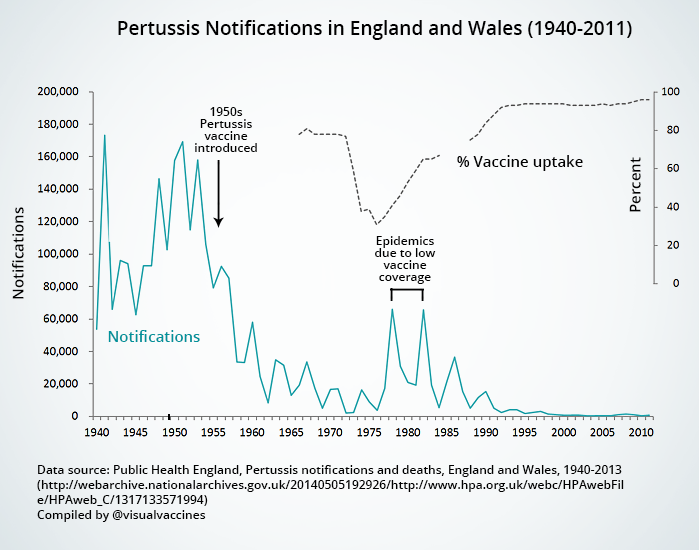
\includegraphics[scale=0.4]{ukpertussis}
\end{center}


\section{Description of the Model}

\subsection{SIR Model}

We used an SIR model for the simulation of the spreading of Pertussis. Pertussis is transmitted by respiratory droplets human-to-human with an incubation period ranging from 9 to 14 days, while symptoms can last up to 6 weeks. \footnote{Torres Codeço, C; Mendes Luz, P; Is pertussis actually reemerging? Insights from an individual-based model, Cad. Saúde Pública vol.17 no.3 Rio de Janeiro May/June 2001}

\subsection{Vaccination Decision}

We assume that every person is a rational decision maker, who decides whether or not to get vaccinated based on the perceived costs of getting vaccination vs risking getting sick. We assume that the vaccination provides 100\% safety, equal to having recovered from the disease. However, as recent research has shown that the protection considerably decreases about 10 to 40 years after the initial protection (vaccination or recovery). \footnote{INSERT RESEACH ABOUT 12 YEARS HERE} To include this in our model without further complicating it, we modelled that the protection stops 12 years after the last immunisation, 

has an initial inclination to vaccinate themselves, which we initialise before the simulation. 

\subsection{Important Parameters}
First we look at the dynamics of the disease. Pertussis is highly contagious, and is transmitted via the respiratory organs. Sneezing, coughing or even speaking can release enough infected particles to cause the disease, making crowded spaces such as public transport and educational institutions ideal for transmission. We therefore initialised everyone in the network to have 40 connections, of which he or she meets 40\% every day, which seems realistic given that even a short encounter on a train station might cause the disease. 
\begin{lstlisting}
#Random probability (per day and person) to become sick 
#without being infected by someone else
prob_for_diseases = 0.00003 

#probability to infect someone when there is contact
prob_for_contact_infection = 0.5 

#incubation time (in days)
incubation_time = 10
 
#days from infection, after this time a person is recovered
time_to_get_healthy = 10 
\end{lstlisting}

\section{Implementation}
The model was implemented using Python. First, we wrote the basic SIR model with infection and recovery. Then we added the "vaccination function" which returns whether a person is getting vaccinated or not. Finally, 

\vspace{14px}



\subsection{SIR Model Implementation}


\section{Simulation Results and Discussion}

\subsection{Limitations}

\subsection{Algorithm Performance}

\section{Summary and Outlook}

\section{References}
Table of References: 
\vspace{14px}

Bauch, C. T., \& Earn, D. J. (2004). Vaccination and the theory of games. Proceedings of the National Academy of Sciences, 101(36), 13391-13394.
\vspace{14px}

Eshel, I. (1996). On the changing concept of evolutionary population stability as a reflection of a changing point of view in the quantitative theory of evolution. Journal of mathematical biology, 34(5-6), 485-510.
\vspace{14px}

Heal, G., \& Kunreuther, H. (2005). The vaccination game. Risk Management and Decision Processes Center Working Paper, (05-10). 
\vspace{14px}

Torres Codeço, C; Mendes Luz, P; Is pertussis actually reemerging? Insights from an individual-based model, Cad. Saúde Pública vol.17 no.3 Rio de Janeiro May/June 2001
\vspace{14px}

$https://ourworldindata.org/vaccination$ 
\vspace{14px}

$https://www.gapminder.org/data/$ search for 'vaccine'
\vspace{14px}

Immunization coverage, system indicators and schedule, and disease incidence $www.who.int/immunization/monitoring_surveillance/data/en$


\newpage




\end{document}  



 
